\documentclass[tikz,border=3pt]{standalone}
\usepackage[utf8]{inputenc}
\usepackage[T1]{fontenc}
\usepackage{lmodern}
\renewcommand{\familydefault}{\sfdefault}
\usepackage{sansmath}\sansmath
\usepackage{chemfig}
\usepackage{pgfplots}\pgfplotsset{compat=1.18,/pgf/number format/use comma,/pgf/number format/1000 sep={.}}
\usetikzlibrary{arrows.meta,calc,positioning,decorations.pathmorphing,patterns}
% paleta del sitio
\definecolor{nar}{HTML}{E8680C}\definecolor{narc}{HTML}{FFB35C}\definecolor{hielo}{HTML}{FFF3E8}
\definecolor{tinta}{HTML}{1D1D1F}\definecolor{gris}{HTML}{6E6E73}\definecolor{lila}{HTML}{7C5CF0}
\definecolor{azul}{HTML}{2F6FD6}\definecolor{menta}{HTML}{17A673}\definecolor{coral}{HTML}{E8342A}
\begin{document}
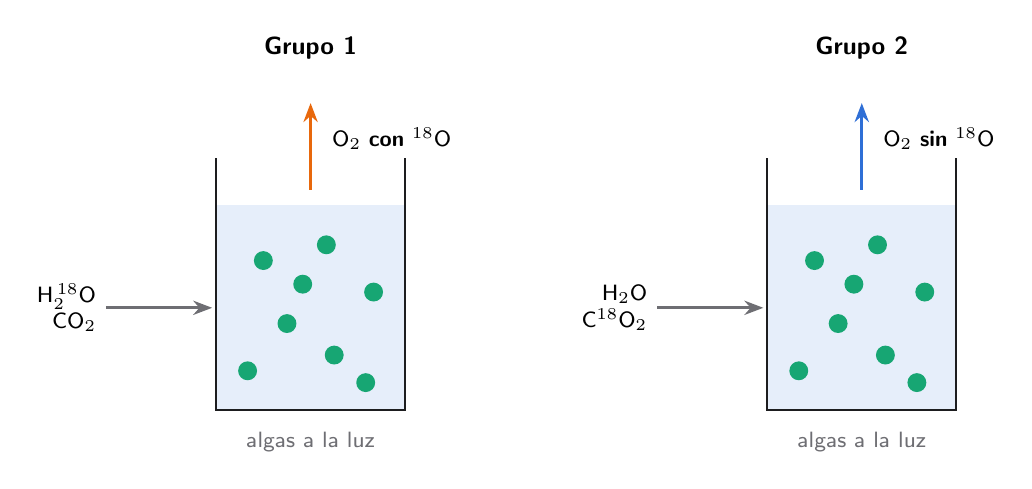
\begin{tikzpicture}[font=\small,>={Stealth[length=2.4mm]}]
\foreach \X/\G/\agua/\co/\res/\col in {0/1/H$_2^{\,18}$O/CO$_2$/O$_2$ \textbf{con} $^{18}$O/nar,7/2/H$_2$O/C$^{18}$O$_2$/O$_2$ \textbf{sin} $^{18}$O/azul}{
\begin{scope}[shift={(\X,0)}]
\node[font=\small\bfseries] at (2,4.6) {Grupo \G};
\fill[azul!12] (0.8,0) rectangle (3.2,2.6);
\draw[tinta,thick] (0.8,3.2) -- (0.8,0) -- (3.2,0) -- (3.2,3.2);
\foreach \x/\y in {1.2/0.5,1.7/1.1,2.3/0.7,2.8/1.5,1.4/1.9,2.2/2.1,2.7/0.35,1.9/1.6} \fill[menta] (\x,\y) circle (0.12);
\node[align=center,font=\footnotesize,text=gris] at (2,-0.4) {algas a la luz};
\draw[->,very thick,gris] (-0.6,1.3) -- (0.75,1.3);
\node[anchor=east,align=right,font=\footnotesize] at (-0.6,1.3) {\agua\\\co};
\draw[->,very thick,\col] (2,2.8) -- (2,3.9);
\node[anchor=west,font=\footnotesize] at (2.15,3.45) {\res};
\end{scope}}
\end{tikzpicture}
\end{document}
